

\begin{figure}[t]
    \centering
    \begin{tabular}{cc}
        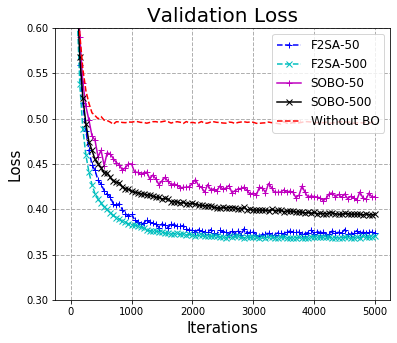
\includegraphics[width=75mm]{Figures/corrupt=0.1.png} &
        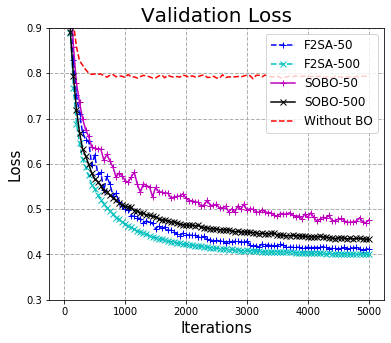
\includegraphics[width=75mm]{Figures/corrupt=0.3.png} \\
        (a) & (b)
    \end{tabular}
    \caption{Outer objective (validation) loss with label corruption rate: (a) $p=0.1$, (b) $p=0.3$.}
    \label{fig:basic_experiment}
\end{figure}

We demonstrate the proposed algorithms on a data hyper-cleaning task involving MNIST \cite{deng2012mnist}.
We are given a noisy training set $\mD_{\text{train}} := \{(\tilde{x}_i, \tilde{y}_i)\}_{i=1}^{n}$ with the label $\tilde{y}_i$ being randomly corrupted with probability $p < 1$. 
We are also given a small but clean validation set $\mD_{\text{val}} := \{(x_i, y_i)\}_{i=1}^{m}$. 
The goal is to assign weights to each training data point so that the model trained on the weighted training set yields good performance on the validation set. 
This task can be formulated as bilevel opimization problem, as follows:
\begin{align*}
    \min_{\lambda} &\qquad \qquad   \tssum_{i=1}^m l(x_i, y_i; w^*) \\
    \text{s.t.}  &\qquad  w^* \in \arg \min_{w} \tssum_{i=1}^n \sigma(\lambda_i) l(\tilde{x}_i, \tilde{y}_i; w) + c \|w\|^2.  
\end{align*}
where $\sigma(\cdot)$ is a sigmoid function, $l(x,y;w)$ is a logistic loss function with parameter $w$ and $c$ is a regularization constant. We use $n=19000$ training samples and $m=1000$ clean validation samples with regularization parameter $c = 0.01$. 
We do not include momentum-assisted methods in our discussion, since we do not observe a significant improvement over the \algname \,
approach of Algorithm~\ref{algo:algo_name} .

We demonstrate the performance of Algorithm \ref{algo:algo_name} (\algname) %\swcomment{Need to change FOBO to \algname \, in the figures} 
and the second-order based method (SOBO) with batch sizes $50$ and $500$. 
We note that several existing second-order methods are in principle the same when momentum or variance-reduction techniques are omitted \cite{ghadimi2018approximation, hong2020two, chen2021closing}, so we use the implementation of stocBiO \cite{ji2021bilevel} as a representative of the other second-order methods.
As a baseline, we also add a result from training without bilevel formulation (Without BO), {\it i.e.,} train on all samples as usual, ignoring the label corruption. 
Results are shown in Figure~\ref{fig:basic_experiment}.\footnote{We report our best results obtained with different hyper-parameters for each algorithm. }

%We remark that we do not intend to compete against second-order methods with convergence speed since in theory, the convergence rate is expected to slow down in terms of iteration counts when only first-order information is accessed. 
Although iteration complexity is worse for first-order methods than SOBO, we observe that \algname~is at least on par with SOBO in this example. 
It can even give superior performance when the batch size is small. 
We conjecture that stochastic noises in Hessian become significantly larger than those in gradients, degrading the performance of SOBO. 
In our experiment, we also observe that Neumann approximation \cite{ghadimi2018approximation} for estimating the Hessian-inverse may induce non-negligible bias in practice.\footnote{We used degree 5 approximation in our experiment. A larger degree approximation did not yield significant improvement.}
In contrast, our fully first-order method \algname~is much less sensitive to small batch sizes and free of bias. 



